%************************************************

\chapter{PAI Cross Section and Optical Constants}

\label{app:cross_section}
%************************************************

\section{Sources for Optical Constants}
The \ac{PAI} cross section in Chapter~\ref{ch:lips} uses the same sources for optical constants as were used in the \ac{CDMS} result \cite{Agnese2015} \cite{Prasad2013}. The sources are outlined in Figure~\ref{fig:const_sources}, along with the cross section for Si.

\begin{figure}[htbp]
\begin{center}
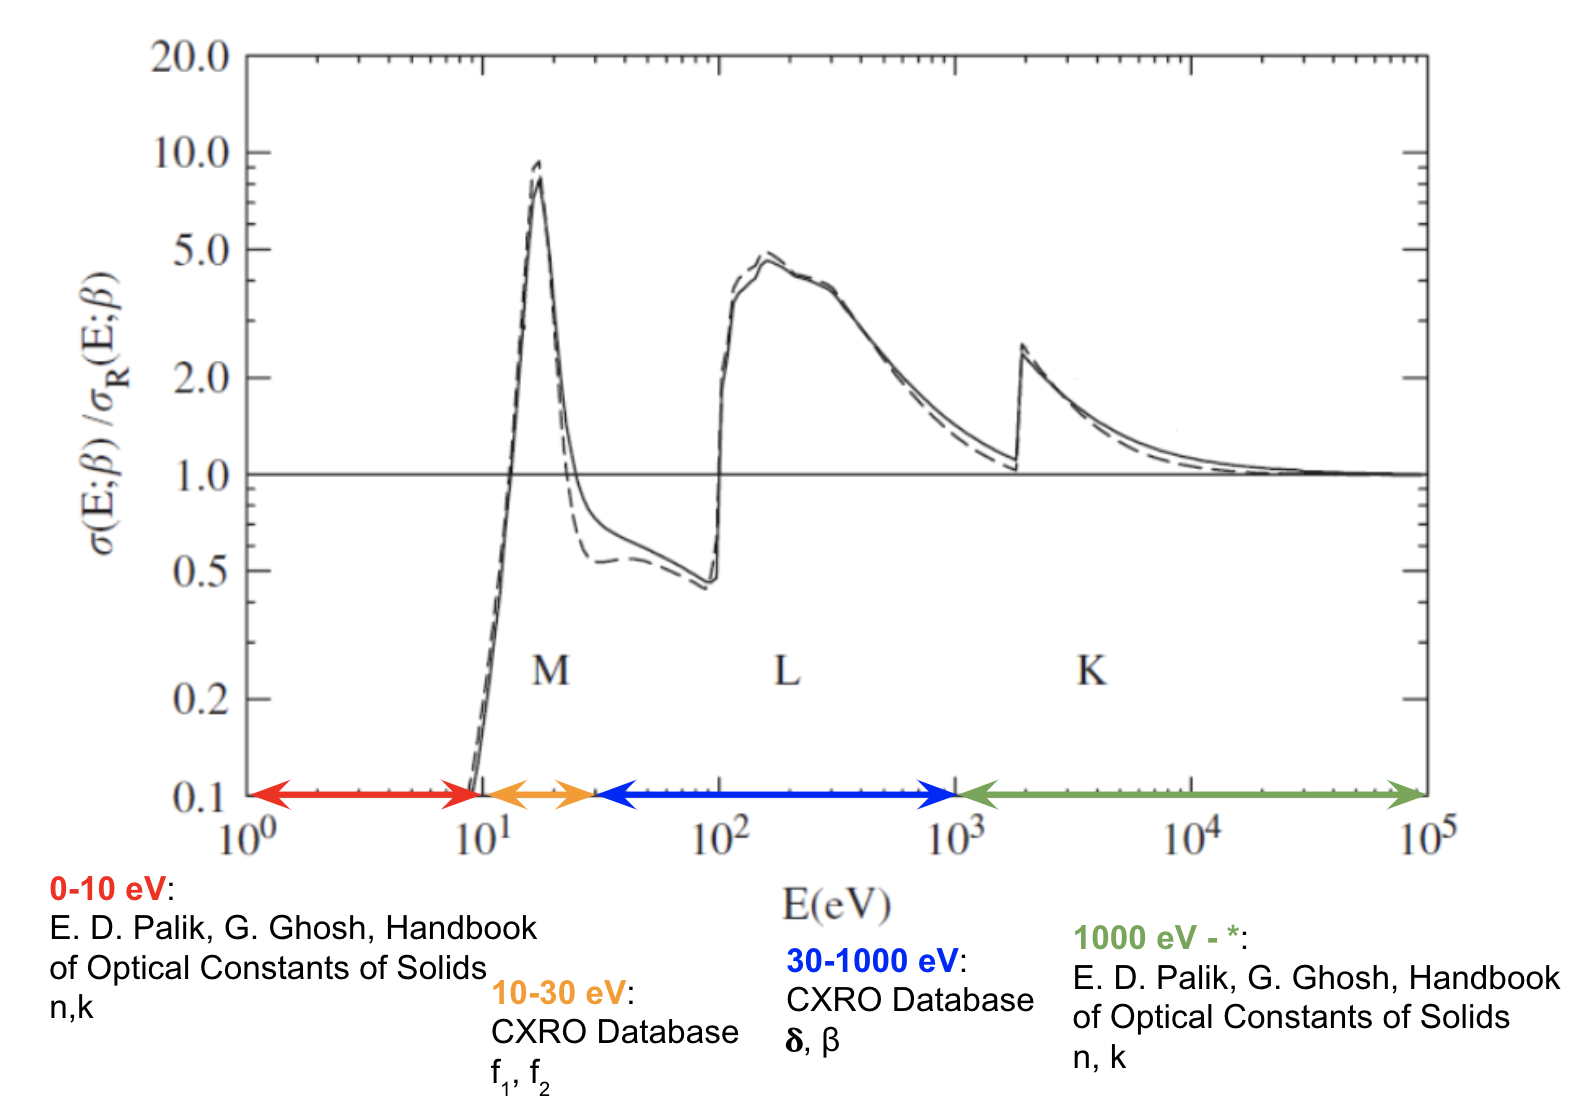
\includegraphics[width=\textwidth]{figures/app/const_sources.png}
\caption{ The sources for the different optical constants used for the \acs{CDMS} \acs{LIP} result and also the \acs{LIP} analysis presented in Chapter~\ref{ch:lips} of this thesis. Figure from \cite{Bichsel:2006}. }
\label{fig:const_sources}
\end{center}
\end{figure}

Dresselhaus \cite{Dresselhaus1966} was the most helpful text in translating these various optical constants into the useful $\epsilon_{1}$ and $\epsilon_{2}$.

Milhay Novak of Geant4 also provided a different set of optical constants, which originated from the EPICS database (this correspondence was over email). The two results are shown in Figure~\ref{fig:pai_different_consts} for both Si and Xe. All the different combinations of constants and code match for Si, indicating there is no error in my calculation of the cross section. For Xe, the EPICS constants do not appear to match the Palik and CXRO constants.

\begin{figure}[htbp]
\begin{center}
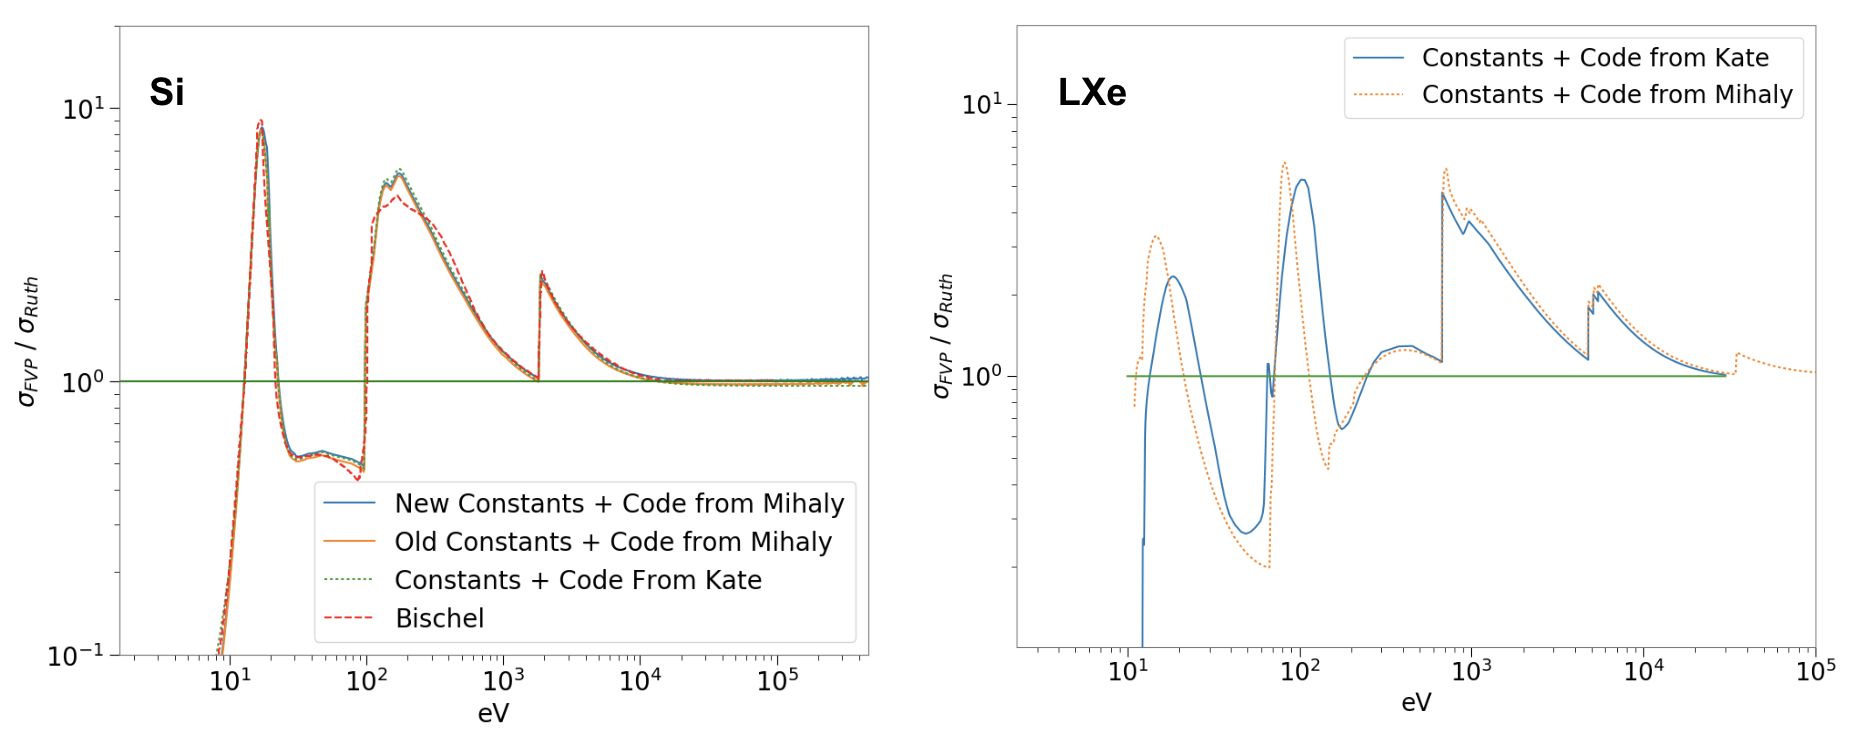
\includegraphics[width=\textwidth]{figures/app/pai_different_consts.png}
\caption{ (left) Plot of the \acs{PAI} cross section divided by the Rutherford cross section for Si. Comparing the different sources for optical constants and calculation method shows that (1) the EPICS constants and the Palik/CXRO match and (2) my code that calculates the \acs{PAI} cross section does not have any obvious errors. (right) Plot of the \acs{PAI} cross section divided by the Rutherford cross section, showing the EPICS and Palik/CXRO constants do not match for Xe.}
\label{fig:pai_different_consts}
\end{center}
\end{figure}

The 1D base straggling Monte Carlo described in Chapter~\ref{ch:lips} was compared for both the EPICS and Palik/CXRO versions of the Xe cross section. There wasn't a measurable difference in the $\langle dE/dx \rangle$, and the same 13\% error when compared to \cite{PDG} was present.

Both the Palik/CXRO and EPICS versions of the cross section for Xe are tabulated below.

\section{PAI Cross Section}
Need to figure out if I can attach a data file to the thesis. 
